\documentclass{article}
\usepackage{header} % Required for inserting images
% \newcommand{\p}[1]{$\mathbb{P}(#1)$}


\title{\LARGE{Теория вероятностей и математическая статистика—1}\\
Теоретический и задачный минимумы\\
ФЭН НИУ ВШЭ}
\author{Винер Даниил  \href{https://t.me/danya_vin}{@danya\_vin}}
\date{Версия от \today}

\begin{document}
\maketitle
\tableofcontents
\newpage
\setlength{\parindent}{15pt}
\setlength{\parskip}{2mm}
\setlist[itemize]{left=1cm}
\setlist[enumerate]{left=1cm}
\section{Теоретический минимум}
% \subsection{Сформулируйте классическое определение вероятности}
% Имеет место, когда исходы равновероятны

% Пусть $\Omega$ — пространство элементарных исходов, то есть все события, которыми может закончиться эксперимент\\
% $\Omega=\{\omega_1,\omega_2,\ldots,\omega_n\}$

% \definition Случайное событие $A$ — любое подмножетсво $\Omega$, причем только для счетных и менее множеств

% \definition
% $$P(A)=\displaystyle\frac{|A|}{|\Omega|}$$

% \definition $P(A)=\sum_{\omega_i\in A}p(\omega_i)$
% \subsection{Выпишите формулу условной вероятности}
% $P(A|B)=\displaystyle\frac{P(A\cap B)}{P(B)}\ \forall B: P(B)>0$

% \subsection{Дайте определение независимости (попарной и в совокупности) для $n$ случайных событий}
% \definition События $A\text{ и }B$ называются \textbf{независимыми}, если:
% \begin{equation*}
%     \begin{aligned}
%         P(A\cap B)&=P(A)\cdot P(B)
%         % \\
%         % P(A|B)P(B)&=P(A)\cdot P(B)\text{ — вытекает интуитивное определение}
%     \end{aligned}
% \end{equation*}

% \definition События $A_1,\ldots, A_n$ \textbf{попарно независимы}, если:
% \begin{equation*}
%     \forall i\ne j\in I,\text{ где $I$ — множество индексов}: \prob{A_i\cap A_j}=\prob{A_i}\cdot\prob{A_j}
% \end{equation*}

% \definition События $A_1,\ldots, A_n$ \textbf{независимы в совокупности}, если:
% \begin{equation*}
%     \begin{aligned}
%     \forall i_1<\ldots<i_k<\ldots<i_n\ \forall k=1,\ldots,n:\\ P(A_{i_1}\cap A_{i_2}\cap\ldots\cap A_{i_k})=P(A_{i_1})\cdot P(A_{i_2})\cdot \ldots\cdot P(A_{i_k})
%     \end{aligned}
% \end{equation*}

% \comment  Для $A_1,A_2,A_3$:
% \begin{equation*}
%     \begin{aligned}
%         P(A_1\cap A_2)&=P(A_1)\cdot P(A_2)\\
%         P(A_2\cap A_3)&=P(A_2)\cdot P(A_3)\\
%         P(A_1\cap A_3)&=P(A_1)\cdot P(A_3)\\
%         P(A_1\cap A_2\cap A_3)&=P(A_1)\cdot P(A_2)\cdot P(A_3)
%     \end{aligned}
% \end{equation*}

% \subsection{Выпишите формулу полной вероятности, указав условия её применимости}
% Пусть $\{H_i\}$ — полная группа несовместных событий (разбиение $\Omega$)

% Должны быть выполнены такие свойства:
% \begin{itemize}
%     \item $H_i\cap H_j=\varnothing\ \forall i\ne j$ — несовместность\\[1mm]
%     \item $\displaystyle\bigcup_{i=1}^{n}H_i=\Omega$ — полнота
% \end{itemize}

% \theorem Тогда, $P(A)=\sum_{i=1}^{n}P(A|H_i)P(H_i)$

% \proof
% \begin{equation*}
%     \begin{aligned}
%         P(A)&=P\left(\bigcup_{i=1}^{n}(A\cap H_i)\right)\\
%         &=\sum_{i=1}^{n}P(A\cap H_i)\\
%         &=\sum_{i=1}^{n} P(A|H_i)\cdot P(H_i)
%     \end{aligned}
% \end{equation*}\qed

% \subsection{Выпишите формулу Байеса, указав условия её применимости}
% Пусть $H_1, H_2, \ldots$ — полная группа несовместных событий, для которой выполняются критерии полноты и несовместности (см. предыдущий пункт), и $A$ — некоторое событие, вероятность которого положительна. При этом, $H_i\ne\varnothing$

% Тогда условная вероятность того, что имело место событие $H_k$, если в резулътате эксперимента наблюдалось событие $A$, может быть вычислена по формуле
% \begin{equation*}
%     \begin{aligned}
%         P(H_k|A)&=\frac{P(A|H_k)\cdot P(H_k)}{P(A)}\\
%         &=\frac{P(H_k\cap A)}{P(A)}\\
%         &=\frac{P(A|H_k)\cdot P(H_k)}{\sum_{i=1}^{n} P(A|H_i)P(H_i)}
%     \end{aligned}
% \end{equation*}


\subsection{Дайте определение функции распределения $F_X (x)$ случайной величины $X$. Укажите необходимые и достаточные условия для того, чтобы функция была функцией распределения некоторой случайной величины}
\definition Функцией рапсредделния случайной величины $X$ называется функция 
\begin{equation*}
    F_X(x):=\prob{X\leqslant x},x\in\mathbb{R}
\end{equation*}

\theorem Функция $G:\mathbb{R}\to[0;1]$ является функцией распределения некоторой случайной величины $\xi\Longleftrightarrow$
\begin{itemize}
    \item $G(x)$ является нестрого возрастающей, то есть $\forall x_1,x_2, x_1\leqslant x_2\ G(x_1)\leqslant G(x_2)$
    \item $G(x)$ является непрерывной справа в каждой точке $x\in\mathbb{R}$, то есть $\forall x\in\mathbb{R}\ \lim\limits_{y\to x+0} G(y)=G(x)$
    \item $\lim\limits_{x\to-\infty} G(x)=0$ и $\lim\limits_{x\to+\infty} G(x)=1$
\end{itemize}

\subsection{Дайте определение функции плотности $f_X (x)$ случайной величины $X$. Укажите необходимые и достаточные условия для того, чтобы функция была функцией плотности некоторой случайной величины}
\definition Говорят, что случайная величина $X$ является абсолютно непрерывной, если ее функция распределения $F_{X}(x)$ представима в виде
\begin{equation*}
    F_X(x):=\int\limits_{-\infty}^{x}f_X(t)\d{t},x\in\mathbb{R},
\end{equation*}
где $f_X(t)$ — неотрицательная интегрируемая функция, которая называется \textit{плотностью распределения} случайной величины $X$

\theorem Функция $g:\mathbb{R}\to[0;+\infty)$ является плотностью распределения некоторой случайной величины $\xi$ тогда и только тогда, когда $\displaystyle\int\limits_{-\infty}^{+\infty} g(x)\d{x}=1$

\subsection{Дайте определение математического ожидания для дискретных и абсолютно непрерывных случайных величин. Укажите, чему равно $\matwait{\alpha X+\beta Y}$, где $X$ и $Y$ — случайные величины, а $\alpha$ и $\beta$ — произвольные константы}
\definition Пусть дискретная случайная величина $X$ принимает значения $a_1,a_2,\ldots,a_k,\ldots$ и ряд 
\begin{equation*}
    \sum_{k=1}^{\infty}|a_k|\cdot\prob{X=a_k}
\end{equation*}
сходится

Тогда, математическим ожиданием случайной величины $X$ называется
\begin{equation*}
    \matwait{X}=\sum_{k=1}^{\infty}a_k\cdot\prob{X=a_k}
\end{equation*}

\definition Пусть случайная величина $X$ является абсолютно непрерывной и интеграл
\begin{equation*}
    \int\limits_{-\infty}^{+\infty}|x|f_{X}(x)\d{x}
\end{equation*}
сходится

Тогда, математическим ожиданием случайной величины $X$ называется 
\begin{equation*}
    \matwait{X}=\int\limits_{-\infty}^{+\infty}xf_X(x)\d{x}
\end{equation*}

\theorem Пусть случайные величины $X$ и $Y$ имеют конечное математическое ожидание\\
Тогда, $\forall \alpha,\beta\in\mathbb{R}$ случайная величина $\alpha X+\beta Y$ тоже имеет конечное математичское ожидание и 
\begin{equation*}
    \matwait{\alpha X+\beta Y}=\alpha\matwait{X}+\beta\matwait{Y}
\end{equation*}

\subsection{Дайте определение дисперсии случайной величины. Укажите, чему равно $\dispersia{\alpha X+\beta}$, где $X$ — случайная величина, а $\alpha$ и $\beta$ — произвольные константы}
\definition Пусть случайная величина $X$ имеет конечное математическое ожидание, тогда дисперсией случайной величины $X$ называется 
\begin{equation*}
    \dispersia{X}=\matwait{(X-\matwait{X})^2}
\end{equation*}

\theorem Пусть случайная величина $X$ имеет конечное математическое ожидание, тогда $\forall \alpha,\beta\in\mathbb{R}$
\begin{equation*}
    \dispersia{\alpha X+\beta}=\alpha^2\dispersia{X}
\end{equation*}


\subsection{Укажите математическое ожидание, дисперсию, множество значений, принимаемых с ненулевой вероятностью, а также функцию плотности или функцию вероятности}
\begin{enumerate}
    \item \textbf{Биномиальное.} Случайная величина $X$ имеет биномиальное распределение с параметрами\\ $n\in\mathbb{N},\ p\in(0;1)$, пишут $X\sim Bi(n,p)$, если случайная величина $X$ принимает значения $0,1,2,\ldots,n$ с вероятностями 
    \begin{itemize}
        \item $\prob{\xi=k}=C_n^k p^k (1-p)^{n-k}$, где $k=0,1,\ldots,n$
        \item $\matwait{\xi}=np$
        \item $\dispersia{\xi}=np(1-p)$
    \end{itemize}
    \item \textbf{Пуассоновское.} Случайная величина $X$ имеет распределение Пуассона с параметром $\lambda>0$, пишут $X\sim Pois(\lambda)$, если случайная величина $X$ принимает значения с вероятностями
    \begin{itemize}
        \item $\prob{\xi=k}=\displaystyle\frac{\lambda^k}{k!}e^{-\lambda}$, где $k\in\{0,1,\ldots\}$
        \item $\matwait{\xi}=\lambda$
        \item $\dispersia{\xi}=\lambda$
    \end{itemize}
    \item \textbf{Геометрическое.} Случайная величина $X$ имеет геометрическое распределение с параметром $p\in(0;1)$, пишут $X\sim Geom(p)$, если случайная величина $X$ принимает значения $k\in\{1,2,3,\ldots\}$ с вероятностями
    \begin{itemize}
        \item $\prob{\xi=k}=p(1-p)^{k-1}$
        \item $\matwait{\xi}=\displaystyle\frac{1}{p}$
        \item $\dispersia{\xi}=\displaystyle\frac{1-p}{p^2}$
    \end{itemize}
    \item \textbf{Равномерное.} Случайная величина $X$ имеет равномерное распределение на отрезке $[a;b]$, где $a<b$, пишут $X\sim U[a;b]$, если случайная величина $X$ имеет плотность 
    \begin{itemize}
        \item $f_{\xi}(x)=\begin{cases}
            \frac{1}{b-a},&\text{ если }x\in[a;b]\\
            0,&\text{ если }x\not\in[a;b]
        \end{cases}$
        \item $F_{\xi}(x)=\begin{cases}
            0,&\text{ если }x<a\\
            \frac{x-a}{b-a},&\text{ если }x\in[a;b]\\
            1,&\text{ если }x>b
        \end{cases}$
        \item $\matwait{\xi}=\displaystyle\frac{a+b}{2}$
        \item $\dispersia{\xi}=\displaystyle\frac{(b-a)^2}{12}$
    \end{itemize}
    \item \textbf{Экспоненциальное (показательное).} Случайная величина $X$ имеет экпоненциальное распределение с параметром $\lambda>0$, пишут $X\sim Exp(\lambda)$, если случайная величина $X$ имеет плотность
    \begin{itemize}
        \item $f_{\xi}(x)=\begin{cases}
            \lambda e^{-\lambda x},&x\geqslant0\\
            0,&x<0
        \end{cases}$
        \item $F_{\xi}(x)=\begin{cases}
            1-e^{-\lambda x},&\text{ если }x\geqslant0\\
            0,&\text{ если }x<0
        \end{cases}$
        \item $\matwait{\xi}=\displaystyle\frac{1}{\lambda}$
        \item $\dispersia{\xi}=\displaystyle\frac{1}{\lambda^2}$
    \end{itemize}
\end{enumerate}

\subsection{Сформулируйте определение функции совместного распределения двух случайных величин, независимости случайных величин. Укажите, как связаны совместное распределение и частные распределения компонент случайного вектора}
\definition Совместной функцией распределения случайных величин $X$ и $Y$ называется функция
\begin{equation*}
    F_{X,Y}(x,y):=\twoprob{X\leqslant x}{\cap}{Y\leqslant y}, x\in\mathbb{R},y\in\mathbb{R}
\end{equation*}

\definition Случайные величины $X$ и $Y$ независимы, если $\forall B_1,B_2\in\bk(\mathbb{R})$ события $\{X\in B_1\}$ и $\{Y\in B_2\}$ являются независимыми, то есть
\begin{equation*}
    \twoprob{X\in B_1}{\cap}{Y\in B_2}=\prob{X\in B_1}\cdot\prob{Y\in B_2}
\end{equation*}

\theorem Случайные величины $X$ и $Y$ независимы тогда и только тогда, когда
\begin{equation*}
    F_{X,Y}(x,y)=F_{X}(x)\cdot F_{Y}(y),\ \forall x\in\mathbb{R},\forall y\in\mathbb{R}
\end{equation*}

\theorem
\begin{enumerate}
    \item $F_{\xi}(x)\in[0;1]$. Здесь и далее $x=(x_1,\ldots,x_n)$
    \item $\lim\limits_{x_1\rightarrow-\infty}F_{\xi}(x_1,x_2)=0$
    
    $\lim\limits_{x_1\rightarrow+\infty}F_{\xi}(x_1,x_2)=F_{\xi_2}(x_2)$

    $\lim\limits_{\underset{x_2\rightarrow+\infty}{x_1\rightarrow+\infty,}}F_{\xi}(x_1,x_2)=1$
    \item $F_{\xi}(x_1,x_2)$ не убывает по каждому из аргументов
    \item $F_{\xi}(x_1,x_2)$ непрерынва справа по каждому из аргументов
\end{enumerate}

\subsection{Сформулируйте определение совместной функции плотности двух случайных величин. Укажите необходимые и достаточные условия для того, чтобы функция была совместной функцией плотности некоторой пары случайных величин. Сформулируйте определение независимости случайных величин}
\definition Случайный вектор $(X,Y)$ имеет абсолютно непрерывное распределение, если совместнаяфункция распределения $F_{X,Y}(x,y)$ представима в виде
\begin{equation*}
    F_{X,Y}(x,y)=\int\limits_{-\infty}^{x}\int\limits_{-\infty}^{y} f_{X,Y}(s,t)\d{s}\d{t},\ \forall x,y\in\mathbb{R},
\end{equation*}
где $f_{X,Y}(s,t)$ — неотрицательная интегрируемая функция, называемая плотностью распределения случайного вектора $(X,Y)$

\theorem Функция $g:\mathbb{R}^2\to[0;+\infty)$ является плотностью распределения случайного вектора $(X,Y)\Longleftrightarrow$
\begin{equation*}
    \iint\limits_{\mathbb{R}^2}g(x,y)\d{x}\d{y}=1
\end{equation*} 

\theorem (в дискретном случае). Пусть случайная величина $X$ принимает значения $a_1,\ldots,a_m$, случайная величина $Y$ принимает значения $b_1,\ldots,b_n$, тогда случайные величины $X$ и $Y$ независимы $\Longleftrightarrow \forall i\in\{1,\ldots,m\},\forall j\in\{1,\ldots,n\}$ события $\{X=a_i\}$ и $\{Y=b_j\}$ независимы, то есть
\begin{equation*}
    \twoprob{X=a_i}{\cap}{Y=b_j}=\prob{X=a_i}\cdot\prob{Y=b_j}
\end{equation*}

\theorem (в абсолютно непрерывном). Пусть случайный вектор $(X,Y)$ имеет абсолютно непрерывное распредедение. Тогда, случайные величины $X$ и $Y$ независимы $\Longleftrightarrow$
\begin{equation*}
    f_{X,Y}(x,y)=f_X(x)\cdot f_{Y}(y),\forall x\in\mathbb{R},\forall y\in\mathbb{R}
\end{equation*}

% \theorem
% \begin{enumerate}
%     \item $F_{\xi}(x)\in[0;1]$. Здесь и далее $x=(x_1,\ldots,x_n)$
%     \item $\lim\limits_{x_1\rightarrow-\infty}F_{\xi}(x_1,x_2)=0$
    
%     $\lim\limits_{x_1\rightarrow+\infty}F_{\xi}(x_1,x_2)=F_{\xi_2}(x_2)$

%     $\lim\limits_{\underset{x_2\rightarrow+\infty}{x_1\rightarrow+\infty,}}F_{\xi}(x_1,x_2)=1$
%     \item $F_{\xi}(x_1,x_2)$ не убывает по каждому из аргументов
%     \item $F_{\xi}(x_1,x_2)$ непрерынва справа по каждому из аргументов
% \end{enumerate}


\newpage
\section{Задачный минимум}
Заметьте, что обозначения $P(\ldots)$ и $\prob{\ldots}$ — это одно и то же, я просто еще не везде исправил
% \subsection{$P(A)=0.3,P(B)=0.4,P(A\cap B)=0.1$}
% \begin{enumerate}
%     \item[\textbf{a)}] Найдите $P(A|B)$
    
%     $P(A|B)=\displaystyle\frac{P(A\cap B)}{P(B)}=\frac{0.1}{0.4}=0.25$
%     \item[\textbf{b)}] Найдите $P(A\cup B)$
    
%     $P(A\cup B)=P(A)+P(B)-P(A\cap B)=0.3+0.4-0.1=0.6$
%     \item[\textbf{c)}] Являются ли события $A$ и $B$ независимыми?

%     \definition События $A$ и $B$ называются независимыми, если $P(A\cap B)=P(A)\cdot P(B)$

%     \definition События $A$ и $B$ называются несовместными, если $A\cap B=\varnothing$

%     Давайте просто проверим, выполняется ли равенство $\prob{A\cap B}=\prob{A}\cdot\prob{B}$:
%     $$\begin{aligned}
%         \prob{A\cap B}&=\prob{A}\cdot\prob{B}\\
%         0.1&=0.3\cdot0.4\\
%         0.1&\ne0.12
%     \end{aligned}$$
%     Это неверно, поэтому события $A$ и $B$ зависимы
%     % Пусть $P(A)\ne0,P(B)\ne0$. Тогда, $A$ и $B$ несовместны, то $A$ и $B$ зависимы

%     % $$0=P(A\cap B)=P(A)\cdot P(B)\ne0\Longrightarrow A \text{ и } B \text{ зависимы}$$
% \end{enumerate}

% \subsection{Карлсон выложил кубиками слово КОМБИНАТОРИКА...}
% \subsubsection*{Способ №1 (С помощью формулы умножения вероятностей)}
% $P(A_1\cap \ldots \cap A_n)=P(A_1)\cdot P(A_2|A_1)\cdot P(A_3|A_1\cap A_2)\cdot\ldots\cdot P(A_n|A_1\cap\ldots\cap A_{n-1})$



% Пусть имеются такие события: \begin{equation*}
%     \begin{aligned}
%         A_1&:=\{\text{первая буква — К}\}\\
%         A_2&:=\{\text{вторая буква — О}\}\\
%         A_3&:=\{\text{третья буква — Р}\}\\
%         A_4&:=\{\text{четвертая буква — Т}\}
%     \end{aligned}
% \end{equation*}

% Тогда, искомая вероятность:
% \begin{equation*}
% \begin{aligned}
%     P(A_1\cap A_2\cap A_3\cap A_4)&=P(A_1)\cdot P(A_2|A_1)\cdot P(A_3|A_1\cap A_2)\cdot P(A_4|A_1\cap A_2\cap A_3)\\
%     &=\frac{2}{13}\cdot\frac{2}{12}\cdot\frac{1}{11}\cdot\frac{1}{10}\\
%     &=\frac{1}{4290}
%     \end{aligned}
% \end{equation*}

% \subsubsection*{Способ №2 (комбинаторный)}
% $P(A)=\displaystyle\frac{|A|}{|\Omega|},\ \Omega=\{(a_1,a_2,a_3,a_4):a_1\in L, a_2\in L, a_3\in L, a_4\in L, a_i\ne a_j\text{ при }i\ne j\}$

% $|\Omega|=\displaystyle\frac{13!}{9!}=17160$

% $A=\{(K_1,O_1,P_1,T_1),(K_2,O_1,P_1,T_1),(K_1,O_2,P_1,T_1),(K_2,O_2,P_1,T_1)\}\longrightarrow$ 4 исхода

% Индекс у букв означают какой по счету встретилась буква в слове <<КОМБИНАТОРИКА>>

% Тогда, искомая вероятность$=\displaystyle\frac{|A|}{|\Omega|}=\frac{4}{17160}=\frac{1}{4290}$

% \subsection{В первой урне 7 белых и 3 черных шара, во второй — 8 белых и 4 черных шара, в третьей — 2 белых и 13 черных шаров}
% $D_i:=\{\text{выбираем $i$-ю урну}\}$, где $i=1,2,3$ — разбиение $\Omega$

% Заметим, что урну мы выбираем равновероятно, то есть $P(D_1)=P(D_2)=P(D_3)=\displaystyle\frac{1}{3}$
% \begin{enumerate}
%     \item[\textbf{a)}] Вычислите вероятность того, что шар, взятый наугад из выбранной урны, окажется белым
    
%     \textbf{Формуа полной вероятности}
%     $$P(A)=P(A|D_1)\cdot P(D_1)+\ldots+P(A|D_n)\cdot P(D_n)$$
%     В нашем случае, формула будет иметь вид
%     $$P(A)=P(A|D_1)\cdot P(D_1)+P(A|D_2)\cdot P(D_2)+P(A|D_3)\cdot P(D_3)$$
%     $A:=\{\text{шар оказался белым}\}$

%     Заметим, что $P(A|D_1)=\frac{7}{10},P(A|D_2)=\frac{2}{3},P(A|D_3)=\frac{2}{15}$, тогда
%     \begin{equation*}
%         \begin{aligned}
%             P(A)&=P(A|D_1)\cdot P(D_1)+P(A|D_2)\cdot P(D_2)+P(A|D_3)\cdot P(D_3)\\
%             &=\frac{7}{10}\cdot\frac{1}{3}+\frac{2}{3}\cdot\frac{1}{3}+\frac{2}{15}\cdot\frac{1}{3}\\
%             &=\frac{1}{2}
%         \end{aligned}
%     \end{equation*}
%     \item[\textbf{b)}] $P(D_1|A)=\displaystyle\frac{P(A|D_1)\cdot P(D_1)}{P(A|D_1)P(D_1)+P(A|D_2)P(D_2)+P(A|D_3)P(D_3)}=\frac{7}{15}$
% \end{enumerate}

% \subsection{В операционном отделе банка работает 80\% опытных сотрудников и 20\% неопытных}
% Обозначим сотрудников так:
% \begin{equation*}
%     \begin{aligned}
%         D_1&:=\{\text{\textbf{опытный} сотрудник}\}\\
%         D_2&:=\{\text{\textbf{неопытный} сотрудник}\}
%     \end{aligned}
% \end{equation*}

% Пусть $A:=\{\text{совершена ошибка}\}$

% Тогда, условия задачи можно записать так:
% \begin{equation*}
%     \begin{aligned}
%         \prob{A|D_1}&=0.01\\
%         \prob{A|D_2}&=0.1
%     \end{aligned}
% \end{equation*}

% \begin{enumerate}
%     \item[\textbf{a)}] $\prob{A}=\prob{A|D_1}\cdot \prob{D_1}+\prob{A|D_2}\cdot \prob{D_2}=0.01\cdot0.8+0.1\cdot0.2=0.028$
%     \item[\textbf{b)}] $\prob{D_2|A}=\displaystyle\frac{\prob{A|D_2}\cdot \prob{D_2}}{\prob{A}}=0.714$

%     Если мы посчитаем по формуле Байеса $\prob{D_1|A}$, то получим, что $(D_2|A)$ и $(D_1|A)$ образуют полную группу вероятностей, то есть $$P(D_2|A)+P(D_1|A)=1\Longrightarrow P(D_1|A)=0.286$$
% \end{enumerate}

% \subsection{Пусть случайная величина $X$ имеет таблицу распределения}
% \begin{table}[h]
%     \begin{tabular}{|c|c|c|c|}
%         \hline
%         $x$ & -1 & 0 & 1 \\
%         \hline
%         $\mathbb{P}(\{X = x\})$ & $0.25$ & $c$ & $0.25$ \\
%         \hline
%     \end{tabular}
% \end{table}

% \begin{itemize}
%     \item[\textbf{а)}] $\Omega = \{X=-1\} + \{X = 0\} + \{X = 1\} \text{ и } 1 = \prob{\{X=-1\}} + \prob{\{X=0\}} + \prob{\{X=1\}} \implies c = 0.5$
%     \item[\textbf{б)}]  $\mathbb{P}\{X\geqslant0\} = \mathbb{P}(\{X=0\}\sqcup\{X=1\}) = \mathbb{P}(\{X=0\}) + \mathbb{P}(\{X=1\}) = 0.75$
%     \item[\textbf{в)}]  $\mathbb{P}(\{X<-3\}) = 0$, т.к. $\Omega$ — дискретное пространство, или же $\{X<-3\} = \{\omega\in \Omega: X(\omega)<-3\}$
%     \item[\textbf{г)}]  $\mathbb{P}(\{X\in [-0.5;0.5]\}) = \mathbb{P}(\{X=0\}) = 0.5$, т.к. $\Omega$ — дискретное пространство
% \end{itemize}

% \subsection{Пусть случайная величина $X$ имеет таблицу распределения}


% \begin{itemize}
%     \item[\textbf{а)}] Аналогично предыдущей задаче — $c=0.5$
%     % $F_X(-100) = \mathbb{P}(\{\omega\in\Omega:\xi(\omega)\leqslant -100\}) = 0$

%     % $$\begin{aligned}
%     %     F_X(0.77) &= \mathbb{P}(\{\omega\in\Omega:\xi(\omega)\leqslant 0.77\})\\
%     %     &=\mathbb{P}(\{X\leqslant 0.77\})\\
%     %     &= \mathbb{P}(\{X=-1\}\sqcup\{X=0\}\\
%     %     &= \mathbb{P}(\{X=-1\}) \mathbb{P}(\{X = 0\}\\
%     %     &= 0.75
%     % \end{aligned}$$
%     \item[\textbf{б)}] $\mathbb{E}[X] = -1\cdot0.25 + 0\cdot0.5+1\cdot0.25 = 0$
%     \item[\textbf{в)}] $\mathbb{E}[X^2] = (-1)^2\cdot0.25 + (0)^2\cdot0.5 + (1)^2\cdot0.25 = 0.5$

%     $\mathbb{E}[\sin{(X)}] = \sin(-1)\cdot0.25 + \sin(0)\cdot0.5 + \sin(1)\cdot0.25$
%     \item[\textbf{г)}] $\dispersia{X} \equiv \dispersia{X} := \mathbb{E}[(X-\mathbb{E}[X])^2] = \mathbb{E}[X^2]- \mathbb{E}^2[X]$
%     \item[\textbf{д)}] $\mathbb{E}[|X|] = |-1|\cdot0.25 + |0|\cdot0.25 + |1|\cdot0.25 = 0.5$

% \end{itemize}

% \begin{table}[h]
%     \begin{tabular}{|c|c|c|c|}
%         \hline
%         $x$ & -1 & 0 & 1 \\
%         \hline
%         $\mathbb{P}(\{\xi = x\})$ & $0.25$ & $c$ & $0.25$ \\
%         \hline
%     \end{tabular}
% \end{table}

% \subsection{Пусть случайная величина $X$ имеет биномиальное распределение с параметрами $n = 4$ и $p = 0.75$}
% $X\sim\text{Bi}(n=4,p=\frac{3}{4})$. Напомним, что $\prob{X=k}=C_4^k (\frac{3}{4})^k(\frac{1}{4})^{4-k}$
% \begin{itemize}
%     \item[\textbf{a)}] $\prob{X=0}=C_4^0 \left(\displaystyle\frac{3}{4}\right)^0\left(\displaystyle\frac{1}{4}\right)^{4}=\left(\displaystyle\frac{1}{4}\right)^4$
%     \item[\textbf{б)}] $\prob{X>0}=1-\prob{X=0}=1-\left(\displaystyle\frac{1}{4}\right)^4$
%     \item[\textbf{в)}] $\prob{X<0}=0$, так как количество успехов в биномиальном распределении $\geqslant0$
%     \item[\textbf{г)}] $\matwait{X}=n\cdot p=4\cdot\frac{3}{4}=3$
%     \item[\textbf{д)}] $\dispersia{X}=np(1-p)=\frac{3}{4}$
%     \item[\textbf{е)}] Нужно посчитать наиболее вероятную величину. Всего есть 5 значений — 5 возможных успешных исходов
    
%     $\prob{X=0}=\left(\displaystyle\frac{1}{4}\right)^4$
    
%     $\prob{X=1}=C_4^1\cdot\displaystyle\frac{3}{4}\cdot\left(\frac{1}{4}\right)^3$

%     $\prob{X=2}=C_4^2\cdot\displaystyle\left(\frac{3}{4}\right)^2\cdot\left(\frac{1}{4}\right)^2$

%     $\prob{X=3}=C_4^3\cdot\displaystyle\left(\frac{3}{4}\right)^3\cdot\left(\frac{1}{4}\right)^1$

%     $\prob{X=4}=C_4^4\cdot\displaystyle\left(\frac{3}{4}\right)^4\cdot\left(\frac{1}{4}\right)^0$

% \end{itemize}
% \subsection{Пусть случайная величина $X$ имеет распределение Пуассона с параметром $\lambda= 100$}
% Имеется случайная величина $X\sim\text{Pois}(\lambda=100)$
% \begin{enumerate}
%     \item[\textbf{a)}] $\prob{\{X=0\}}=\displaystyle\frac{\lambda^0}{0!}e^{-\lambda}=e^{-\lambda}=e^{-100}$
%     \item[\textbf{б)}] $\prob{\{X>0\}}=1-\prob{\{x=0\}}=1-e^{-100}$
%     \item[\textbf{в)}] $\prob{\{X<0\}}=\prob{\varnothing}=0$
%     \item[\textbf{г)}] По определению, $\mathbb{E}\left[X\right]=\lambda$. Докажем
%     \begin{equation*}
%         \begin{aligned}
%             \matwait{X}&=\sum_{k=0}^{\infty} k\cdot\prob{\{x=k\}}\\
%             &=\sum_{k=0}^{\infty} k\frac{\lambda^k}{k!}e^{-\lambda}\\
%             &=\sum_{k=1}^{\infty} \frac{\lambda^k}{(k-1)!}e^{-\lambda}\\
%             &=\lambda e^{-\lambda}\sum_{k=1}^{\infty}\frac{\lambda^{k-1}}{(k-1)!}\\
%             &=\left(\sum_{l=0}^{\infty}\frac{\lambda^l}{l!}\right)\lambda e^{-\lambda}\\
%             &=\lambda
%         \end{aligned}
%     \end{equation*}
%     \item[\textbf{д)}] Для того, чтобы посчитать дисперсию $X$ сначала посчитаем мат.ожидание $X^2$, а для этого посчитаем $\matwait{X(X-1)}$:
%     \begin{equation*}
%         \begin{aligned}
%             \matwait{X(X-1)}&=\sum_{k=0}^{\infty} k(k-1)\prob{\{x=k\}}\\
%             &=\sum_{k=2}^{\infty} k(k-1)\frac{\lambda^k}{k!}e^{-\lambda}\\
%             &=\lambda^2e^{-\lambda}\sum_{k=2}^{\infty}\frac{\lambda^{k-2}}{(k-2)!}e^{-\lambda}\\
%             &=\lambda^2e^{-\lambda}\sum_{l=0}^{\infty}\frac{\lambda^{l}}{l!}\\
%             &=\lambda
%         \end{aligned}
%     \end{equation*}
%     Тогда, $\lambda^2=\matwait{X(X-1)}=\matwait{X^2}-\matwait{X}\Longrightarrow\matwait{X^2}=\lambda+\lambda^2$
    
%     Теперь можем выразить дисперсию через известное равенство:
%     \begin{equation*}
%         \dispersia{X}=\matwait{X^2}-\left(\matwait{X}\right)^2=\lambda+\lambda^2-\lambda^2=\lambda
%     \end{equation*}
%     \item[\textbf{e)}] Предположим, что $X=k$ и есть наиболее вероятное значение, принимаемое $X$. При этом, $k\in\{0,1,2,\ldots\}$. Так как $k$ — дискретная, то дифференцированием мы воспользоваться не можем, тогда посчитаем $\displaystyle\frac{\prob{\{X=k+1\}}}{\prob{\{X=k\}}}$:
%     \begin{equation*}
%         \begin{aligned}
%             \frac{\prob{\{X=k+1\}}}{\prob{\{X=k\}}}&=\frac{\frac{\lambda^{k+1}}{(k+1)!}e^{-\lambda}}{\frac{\lambda^{k}}{k!}e^{-\lambda}}\\
%             &=\frac{\lambda}{k+1}\\
%             &=\frac{100}{k+1}
%         \end{aligned}
%     \end{equation*}
%     Теперь проанализируем при каких $k$ это отношение будет больше, меньше или равно $1$:
%     \begin{itemize}
%         \item $\displaystyle\frac{100}{k+1}>1\Longrightarrow k <99$
%         \item $\displaystyle\frac{100}{k+1}<1\Longrightarrow k >99$
%         \item $\displaystyle\frac{100}{k+1}=1\Longrightarrow k =99$
%     \end{itemize}
%     Значит, $99$ и $100$ — наиболее вероятные значения, принимаемые случайной величиной $X$
%     $$
%     \begin{tikzpicture}
%         \draw[black, ->] (0,0) -- (0,2.5) node[black, left] {$\prob{\{X=k\}}$};
%         \draw[black, ->] (0,0) -- (7,0) node[black, right] {$k$};
%         \draw[black, thick] (0,0) -- (2,1);
%         \draw[black, very thick] (2,1) -- (4,1);
%         \draw[black, thick] (4,1) -- (6,0);
%         \draw[black, dashed] (2,0) node[black, below] {$99$} -- (2,1);
%         \draw[black, dashed] (4,0) node[black, below] {$100$} -- (4,1);
%     \end{tikzpicture}
%     $$
% \end{enumerate}
% \subsection{В лифт 10-этажного дома на первом этаже вошли 5 человек}
% \begin{enumerate}
%     \item[\textbf{а)}] Пусть $\xi_i=\begin{cases}
%         1,&\text{если $i$-й \textit{пассажир} вышел на шестом этаже}\\
%         0,&\text{иначе}
%     \end{cases}$. При этом $i\in\{1,2,3,4,5\}$

%     Тогда, $\xi=\xi_1+\ldots+\xi_5$ — число \textit{пассажиров}, которые вышли на шестом этаже

%     Заметим, что $\xi_1,\ldots,\xi_5$ — независимые, а также $\xi_i\sim\text{Be}\left(p=\frac{1}{9}\right)$. Тогда, $\xi\sim\text{Bi}\left(n=5,p=\frac{1}{9}\right)$

%     $\prob{\{\xi>0\}}=1-\prob{\{\xi=0\}}=1-\left(\frac{8}{9}\right)^5$
%     \item[\textbf{б)}] $\prob{\{\xi=0\}}=C_n^k p^k q^{n-k}=C_5^0\left(\frac{1}{9}\right)^0\left(\frac{8}{9}\right)^5=\left(\frac{8}{9}\right)^5$
%     \item[\textbf{в)}] Пусть $\eta_i=\begin{cases}
%         1,&\text{если $i$-й \textit{пассажир} вышел на 6 этаже или выше}\\
%         0,&\text{иначе}
%     \end{cases}$. При этом $i\in\{1,2,3,4,5\}$

%     Тогда, $\eta=\eta_1+\ldots+\eta_5$ — число \textit{пассажиров}, которые вышли на шестом этаже и выше

%     Заметим, что $\eta_1,\ldots,\eta_5$ — независимые, а также $\eta_i\sim\text{Be}\left(p=\frac{5}{9}\right)$. Тогда, $\eta\sim\text{Bi}\left(n=5,p_1=\frac{5}{9}\right)$

%     $\prob{\{\eta=5\}}=C_5^5\cdot p_1^5\cdot q^0=\left(\frac{5}{9}\right)^5$
% \end{enumerate}
% \subsection{При работе некоторого устройства время от времени возникают сбои}
% $\xi_i\sim\text{Pois}(\lambda=3)$ — число сбоев за $i$-е сутки
% \begin{enumerate}
%     \item[\textbf{а)}] \begin{equation*}
%         \begin{aligned}
%             \prob{\{\xi_i>0\}}&=1-\prob{\{\xi_i=0\}}\\
%             &=1-\frac{\lambda^0}{0!}e^{-\lambda}\\
%             &=1-e^{-3}
%         \end{aligned}
%     \end{equation*}
%     \item[\textbf{б)}] Требуется вычислить вероятность того, что за двое суток не произойдет ни одного сбоя. То есть нужно найти вероятность двух событий: $\{\xi_1=0\}$ и $\{\xi_2=0\}$. Заметим, что эти события независимы. Формально:
%     \begin{equation*}
%         \begin{aligned}
%             \prob{\{\xi_1=0\}\cap\{\xi_2=0\}}&=\prob{\{\xi_1=0\}}\cdot\prob{\{\xi_2=0\}}\\
%             &=e^{-3}\cdot e^{-3}
%         \end{aligned}
%     \end{equation*}
% \end{enumerate}


\subsection{Пусть случайная величина $X$ имеет следующую функцию плотности...}
Дана функция плотности $f_{X}(x)=\begin{cases}
    cx,&x\in[0;1]\\
    0,&x\not\in[0;1]
\end{cases}$

Найдите
\begin{itemize}
    \item $F_X(x)=\displaystyle\int\limits_{-\infty}^{x} f_X(t)\d{t}$. Тогда, при $x\to+\infty$
    \begin{equation*}
        \begin{aligned}
            1=\int\limits_{-\infty}^{+\infty} f_X(t)\d{t}&=\int\limits_0^1 ct\d{t}\\
            &=c\cdot\left.\frac{t^2}{2}\right\vert_{t=0}^{t=1}\\
            &=\frac{c}{2}
        \end{aligned}
    \end{equation*}
    $\Longrightarrow c=2$
    \item \theorem Пусть $\xi$ — абсолютно непрерывная случайная величина, тогда $$\forall B\in\bk(\mathbb{R})\ \prob{\xi\in B}=\displaystyle\int\limits_{B}f_{\xi}(t)\d{t}$$
    
    Тогда, в нашем случае
    \begin{equation*}
        \begin{aligned}
            \prob{X\leqslant\frac{1}{2}}&=\prob{X\in(-\infty;\frac{1}{2}]}\\
            &=\int\limits_{B}f_{X}(t)\d{t}\\
            &=\int\limits_{-\infty}^{\frac{1}{2}}f_{X}(t)\d{t}\\
            &=\int\limits_{-\infty}^{\frac{1}{2}}2t\d{t}\\
            &=\left.t^2\right\vert_{t=0}^{t=\frac{1}{2}}\\
            &=\frac{1}{4}
        \end{aligned}
    \end{equation*}
    \item $\prob{X\in[\frac{1}{2};\frac{3}{2}]}=\displaystyle\int\limits_{B}f_{X}(t)\d{t}=\int\limits_{\frac{1}{2}}^{1}2t\d{t}=\left.t^2\right\vert_{t=\frac{1}{2}}^{t=1}=\frac{3}{4}$
    \item $\prob{X\in[2;3]}=\displaystyle\int\limits_{[2;3]}f_{X}(t)\d{t}=0$
    \item $f_{X}(x)=\begin{cases}
        2x,&x\in[0;1]\\
        0,&x\not\in[0;1]
    \end{cases}$

    Теперь рассмотрим три участка:
    \begin{equation*}
        \begin{aligned}
            x<0:& F_{X}(x)=\int\limits_{-\infty}^{x}f_{X}(t)\d{t}=0\\
            0\leqslant x\leqslant 1:& F_{X}(x)=\int\limits_{-\infty}^{x}f_{X}(t)\d{t}=\int\limits_{-\infty}^{0}0\d{t}+\int\limits_{0}^x 2t\d{t}=\left.t^2\right\vert_{t=0}^{t=x}=x^2\\
            x>1:& F_{X}(x)=\int\limits_{-\infty}^{x}f_{X}(t)\d{t}=\int\limits_{-\infty}^0 0\d{t}+\int\limits_{0}^1 f_{X}(t)\d{t}+\int\limits_{1}^x0\d{t}=1
        \end{aligned}
    \end{equation*}

    $F_{X}(x)=\begin{cases}
        0,&x<0\\
        x^2,&x\in[0;1]\\
        1,&x>1
    \end{cases}$
\end{itemize}


\subsection{Пусть случайная величина $X$ имеет следующую функцию плотности...}
Дана функция плотности $f_{X}(x)=\begin{cases}
    cx,&x\in[0;1]\\
    0,&x\not\in[0;1]
\end{cases}$

Найдите
\begin{itemize}
    \item $F_X(x)=\displaystyle\int\limits_{-\infty}^{x} f_X(t)\d{t}$. Тогда, при $x\to+\infty$
    \begin{equation*}
        \begin{aligned}
            1=\int\limits_{-\infty}^{+\infty} f_X(t)\d{t}&=\int\limits_0^1 ct\d{t}\\
            &=c\cdot\left.\frac{t^2}{2}\right\vert_{t=0}^{t=1}\\
            &=\frac{c}{2}
        \end{aligned}
    \end{equation*}
    $\Longrightarrow c=2$

    \item $\matwait{X}=\displaystyle\int\limits_{-\infty}^{\infty}xf_{X}(x)\d{x}=\int\limits_{0}^1 x2x\d{x}=2\int\limits_0^1 x^2\d{x}=2\cdot\left.\frac{x^3}{3}\right\vert_{0}^1=\frac{2}{3}$
    \item $\matwait{X^2}=\displaystyle\int\limits_{-\infty}^{+\infty}xf_{X}(x)\d{x}=\int\limits_{0}^1x^2 2x\d{x}=\frac{1}{2}$
    \item $\dispersia{X}=\displaystyle\frac{1}{2}-\left(\frac{2}{3}\right)^2=\frac{1}{18}$
    \item $\matwait{\sqrt{X}}=\displaystyle\int\limits_{0}^1\sqrt{x}2x\d{x}=\frac{4}{5}$
\end{itemize}

\subsection{Пусть задана таблица совместного распределения случайных величин $X$ и $Y$}
\begin{equation*}
    \begin{tabular}{cccc}
        \hline
        &$Y=-1$&$Y=0$&$Y=1$\\
        \hline
        $X=-1$&0.2&0.1&0.2\\
        $X=1$&0.1&0.3&0.1\\
        \hline
    \end{tabular}
\end{equation*}

Найдите
\begin{itemize}
    \item $\prob{X=-1}=0.2+0.1+0.2=0.5$
    \item $\prob{Y=-1}=0.2+0.1=0.3$
    \item $\twoprob{X=-1}{\cap}{Y=-1}=0.2$ %(пересечение столбца $Y=-1$ и строки $X=-1$)
    \item Проверим, выполняется ли 
    \begin{equation*}
        \begin{aligned}
            \twoprob{X=-1}{\cap}{Y=-1}&=\prob{X=-1}\cdot\prob{Y=-1}\\
            0.2&\ne0.3\cdot0.5
        \end{aligned}
    \end{equation*}
    $\Longrightarrow $ величины $X$ и $Y$ \textit{не} независимы
    \item $F_{X,Y}(-1;0)=\twoprob{X\leqslant-1}{\cap}{Y\leqslant0}=\twoprob{X=-1}{\cap}{Y=-1}+\twoprob{X=-1}{\cap}{Y=0}=0.2+0.1=0.3$
    \item \begin{tabular}{c|c}
        $X$&$\mathbb{P}$\\
        \hline
        $-1$&$0.5$\\
        \hline
        $1$&$0.5$
    \end{tabular}

    \comment Для случайной величины $Y$ таблица распределения выглядит так: \begin{tabular}{c|c}
        $Y$&$\mathbb{P}$\\
        \hline
        $-1$&$0.3$\\
        \hline
        $0$&$0.4$\\
        \hline
        $1$&$0.3$
    \end{tabular}
    \item $F_{X}(x)=\prob{X\leqslant x}=\begin{cases}
        0,&x<-1\\
        0.5,&x\in[-1;1)\\
        1,&x\geqslant 1
    \end{cases}$
    \item $\begin{tikzpicture}
        \draw[black, ->, thick] (-2,0) -- (3,0) node [right] {$x$};
        \draw[black, ->, thick] (0,0) -- (0,2) node [above left] {$F_X(x)$};
        \draw[black, thin] (-1,0.5) -- (1,0.5);
        \fill[black] (-1,0.5) circle (1.5pt);
        \draw[black, thin] (1,1) -- (2.5,1);
        \fill[black] (1,1) circle (1.5pt);
        \draw (1,0.5) circle (1.5pt);
        \draw (-1,0) node [black, below] {$-1$} circle (1.5pt);
        \draw[black] (1,0) node [black, below] {$1$};
        \draw[black] (0,0.5) node [black, left] {$0.5$};
        \draw[black] (0,1) node [black, left] {$1$};
    \end{tikzpicture}$
\end{itemize}

\subsection{Пусть задана таблица совместного распределения случайных величин $X$ и $Y$}
\begin{equation*}
    \begin{tabular}{cccc}
        \hline
        &$Y=-1$&$Y=0$&$Y=1$\\
        \hline
        $X=-1$&0.2&0.1&0.2\\
        $X=1$&0.2&0.1&0.2\\
        \hline
    \end{tabular}
\end{equation*}
Найдите
\begin{itemize}
    \item $\prob{X=1}=0.2+0.1+0.2=0.5$
    \item $\prob{Y=1}=0.2+0.2=0.4$
    \item $\twoprob{X=1}{\cap}{Y=1}=0.2$
    \item Проверим, выполняется ли 
    \begin{equation*}
        \begin{aligned}
            \twoprob{X=1}{\cap}{Y=1}&=\prob{X=1}\cdot\prob{Y=1}\\
            0.2&=0.5\cdot0.4
        \end{aligned}
    \end{equation*}
    $\Longrightarrow $ величины $X$ и $Y$ независимы
    \item $\begin{aligned}
        F_{X}(1;0)&=\twoprob{X\leqslant1}{\cap}{Y\leqslant0}\\
        &=\twoprob{X=-1}{\cap}{Y=-1}+\twoprob{X=-1}{\cap}{Y=0}\\
        &+\twoprob{X=1}{\cap}{Y=-1}+\twoprob{X=1}{\cap}{Y=0}\\
        &=0.2+0.1+0.2+0.1\\
        &=0.6
    \end{aligned}$
    \item \begin{tabular}{c|c}
        $Y$&$\mathbb{P}$\\
        \hline
        $-1$&$0.4$\\
        \hline
        $0$&$0.2$\\
        \hline
        $1$&$0.4$
    \end{tabular}
    \item $F_{Y}(y)=\prob{Y\leqslant y}=\begin{cases}
        0,&y<-1\\
        0.4,&y\in[-1;0)\\
        0.6,&y\in[0;1)\\
        1,&y\geqslant1
    \end{cases}$
    \item $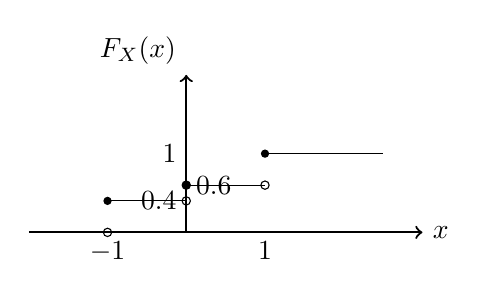
\begin{tikzpicture}
        \draw[black, ->, thick] (-2,0) -- (3,0) node [right] {$x$};
        \draw[black, ->, thick] (0,0) -- (0,2) node [above left] {$F_X(x)$};
        \draw[black, thin] (-1,0.4) -- (0,0.4);
        \draw[black, thin] (1,1) -- (2.5,1);
        \fill[black] (-1,0.4) circle (1.5pt);
        \draw[black, thin] (0,0.6) -- (1,0.6);
        \fill[black] (1,1) circle (1.5pt);
        \draw (0,0.4) node [black, left] {$0.4$} circle (1.5pt);
        \draw[fill=black] (0,0.6) node [black, right] {$0.6$} circle (1.5pt);
        \draw (1,0.6) circle (1.5pt);
        \draw (-1,0) node [black, below] {$-1$} circle (1.5pt);
        \draw[black] (1,0) node [black, below] {$1$};
        \draw[black] (0,1) node [black, left] {$1$};
    \end{tikzpicture}$
\end{itemize}




\end{document}
